%Dies ist die Vorlage für die einzelnen Kapitel, die jeweils mit Chapter als Kapiteltitel starten
\chapter{Sicherheitsniveaus}

Das nachfolgende Kapitel geht auf verschiedene Sicherheitsbedürfnisse eines Nutzers ein. Gerade im Hinblick auf den Grad der Verschlüsselung bei der E-Mail Kommunikation ist es wichtig sich darüber bewusst zu werden, wie sensibel die Information ist, die man versenden möchte. Denn jede Verschlüsselung ist mit einem bestimmten Aufwand verbunden und folglich ist abzuwägen, welcher Verschlüsselungsaufwand dem Nutzer die zu versendende Information wert ist. 
Beispielsweise ist aus Sicht der Autoren der potentielle Schaden gering, wenn eine E-Card zu den Weihnachtsfeiertagen an den nicht rechtmäßigen Empfänger gerät, sodass für die Versendung einer solchen Information der Grad der Verschlüsselung niedrig und somit der Aufwand niedrig ausfällt. Dahingegen ist der potentielle Schaden größer, wenn es sich bei der versendeten Information um beispielsweise die eigenen Kontodaten handelt, was wiederum bedeutet, dass der Nutzer bereit ist einen höheren Aufwand zu betreiben, um diese Inhalte auf eine sichere Art und Weise via E-Mail zu übermitteln.


Das Sicherheitsbedürfnis einer jeden Person kann unterschiedlich stark ausgeprägt sein. Daher ist es den Autoren nicht möglich, eine allgemein gültige Auflistung aller möglichen Szenarien der E-Mail Kommunikation bereitzustellen, aus welcher die Teilnehmer der Zielgruppe lediglich das richtige Szenario heraussuchen müssen und dadurch den optimalen Grad der Verschlüsselung erhalten. Stattdessen wird in Abbildung \ref{img:sicherheitsniveaus} eine Übersicht präsentiert, die es dem Nutzer erlaubt auf Basis seines eigenen Sicherheitsbedürfnisses und mit Hilfe festgelegter Kriterien für die Übermittlung einer ganz bestimmten Information ein geeignetes Sicherheitsniveau zu ermitteln. In den nachfolgenden dieser Arbeit werden verschiedene Möglichkeiten der Verschlüsselung von E-Mail Kommunikation vorgestellt und jeweils passenden Sicherheitsniveaus zugeordnet. Dabei erfolgt diese Zuordnung mit dem Ziel, einen optimalen Ausgleich zwischen Notwendigkeit und Aufwand der Verschlüsselung von E-Mails zu erhalten, sodass der Nutzer nach der Ermittlung eines geeigneten Sicherheitsniveaus eine aus Sicht der Autoren geeignete Verschlüsselungsmethode ermitteln kann.

\pagebreak


\begin{figure}[h] %{wrapfigure}[36]{l}{1.0\textwidth}
	%\begin{center}
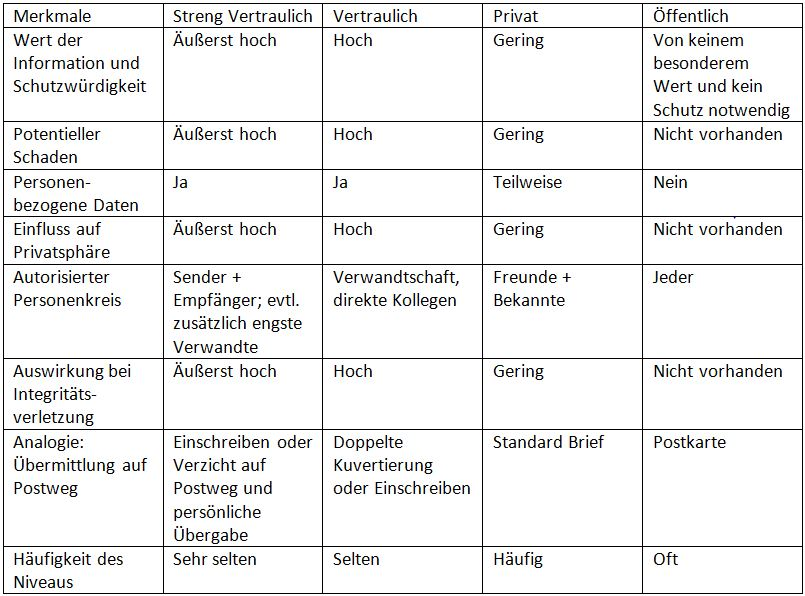
\includegraphics[width=16cm]{images/sicherheitsniveaus.jpg}
	%\end{center}

\caption {Sicherheitsniveaus} %Bildunterschrift, erstes Argument ist für Abbildungsverzeichnis ohne Fußnote; \footnotemark ist ein Platzhalter für die Fußnote
\label{img:sicherheitsniveaus} %für Bezüge auf diese Abbildung

\end{figure} %wrapfigure}


Die Abbildung \ref{img:sicherheitsniveaus} stellt im Tabellenkopf vier verschiedene Sicherheitsniveaus dar: \textit{Streng Vertraulich, Vertraulich, Privat und Öffentlich}. Dabei nimmt das Sicherheitsbedürfnis sowie der Verschlüsselungsaufwand von Streng Vertraulich hin zu Öffentlich ab.
In der ersten Spalte sind verschiedene Merkmale aufgelistet, welche es dem Nutzer ermöglichen sollen, für eine ganz bestimmte Information ein geeignetes Sicherheitsniveau zu bestimmen.
Alle weiteren Felder enthalten die Ausprägung des Merkmals innerhalb des jeweiligen Sicherheitsniveaus.

Der Wert der Information und deren Schutzwürdigkeit beschreiben, wie wertvoll die zu versendende E-Mail für einen nicht rechtmäßigen Empfänger ist und welche Notwendigkeit des Schutzes daraus folgt.
Der potentielle Schaden stellt das Ausmaß dar, welches eintritt für den Fall, dass die E-Mail durch einen unberechtigten Dritte gelesen wird. Dieser Schaden kann verschiedener Art sein. Zum Beispiel können daraus rechtliche Konsequenzen erfolgen, es kann zu einem finanziellen Verlust führen oder mit einer Schädigung des Images des Senders einhergehen \footcite[Vgl.][]{Reinhausen GmbH, S. 6}. Aus dem potentiellen Schaden lässt sich außerdem gut der Einfluss auf die eigene Privatsphäre ableiten.
Das Merkmal \textit{Personenbezogene Daten} besagt, dass die zu versendende Information personenbezogene Daten enthält und daher grundsätzlich das Sicherheitsniveau \textit{Vertraulich} zu wählen ist\footcite[Vgl.][]{TSE}. In Abhängigkeit von der Ausprägung der anderen Merkmale, kann als resultierendes Sicherheitsniveau auch \textit{Streng Vertraulich} oder \textit{Privat} ermittelt werden.
Der Autorisierte Personenkreis ist eine weitere Eigenschaft anhand derer der Nutzer ein passendes Sicherheitsniveau bestimmen kann. Grundsätzlich gilt: je wertvoller die Information, desto geringer ist der Personenkreis, der Einblick in die zu versendende E-Mail erhalten darf \footcite[Vgl.][]{TSE}. Daraus folgt, dass eine streng vertrauliche Nachricht ausschließlich zwischen dem Sender und dem Empfänger ausgetauscht wird und in der Regel keine weitere Person über den Inhalt erfahren darf. Eine Ausnahme an dieser Stelle sind allenfalls engste Verwandte. Dahingegen ist für eine Nachricht, deren Inhalt prinzipiell jedermann erfahren darf, das Sicherheitsniveau \textit{Öffentlich} zu wählen\footcite[Vgl.][]{Reinhausen GmbH, S. 10}.
Die \textit{Auswirkung bei Integritätsverletzung} beschreibt das eingetretene Ausmaß, wenn die E-Mail in die Hände eines Angreifers gelangt ist.
Eine weitere Möglichkeit ein geeignetes Sicherheitsniveau zu ermitteln ist die Überlegung, wie der Inhalt der E-Mail auf dem Postweg versandt werden würde. Für eine streng vertrauliche Information würde ein Einschreiben gewählt werden oder gänzlich auf den Postweg verzichtet und stattdessen die Nachricht persönlich überbracht werden. Dahingegen ist für Information, die ohne Bedenken  auf einer Postkarte übermittelt werden können, das Sicherheitsniveau \textit{Öffentlich} zu wählen 
Das letzte Merkmal beschreibt das Aufkommen der einzelnen Sicherheitsniveaus. Streng vertrauliche Informationen sind sehr selten und am häufigsten werden öffentliche Nachrichten ausgetauscht \footcite[Vgl.][]{TSE}.

Anhand des nachfolgenden Beispiels soll der Umgang mit der Abbildung \ref{img:sicherheitsniveaus} verdeutlicht werden. Hierbei ist zu erwähnen, dass das resultierende Sicherheitsniveau auf Basis des beschriebenen Sicherheitsbedürfnisses ermittelt wurde und für die gleiche Information bei anderen Nutzern unterschiedlich ausfallen kann:

Herr Meier war vor kurzem in einen Auffahrunfall verwickelt, den ein unachtsamer Autofahrer verursacht hatte. Daraufhin brachte Herr Meier sein Fahrzeug in die Werkstatt und ließ ein Gutachten des Schadens erstellen. Dieses Gutachten möchte er nun zusammen mit seinen Kontodaten via E-Mail an die Versicherung des Unfallverursachers senden. 
Der Wert dieser Information ist hoch, denn einerseits sind die Kontodaten in der Nachricht vorhanden. Andererseits ist in dem Gutachten Herr Meiers Anschrift angegeben und es lässt sich aus den Fotos und der Schadenshöhe des Gutachtens ableiten, dass Herr Meier einen Luxuswagen besitzt. Daraus wiederum lassen Rückschlüsse auf seine finanzielle Situation schließen. Der potentielle Schaden, der sich daraus ergibt, ist hoch bis äußerst hoch. Denn bei ausreichender krimineller Energie können nicht nur die Kontodaten missbraucht werden, sondern mit Hilfe der Anschrift kann der Wohnsitz von Herrn Meier ausgekundschaftet und beispielsweise bei seiner Abwesenheit in sein Anwesen eingebrochen werden. 
Die Anschrift stellt personenbezogene Daten dar und ermöglicht einen hohen Einfluss auf die Privatsphäre von Herrn Meier.
Der Autorisierte Personenkreis für diese Nachricht beschränkt sich auf den Sender (Herr Meier), den Empfänger (die Versicherung) sowie auf seine Frau und auf die Werkstatt, die das Gutachten erstellt hat. Seinen Freunden und Kollegen hat Herr Meier zwar auch von dem Unfall erzählt. Allerdings wissen diese keine genaueren Details hinsichtlich des Schadens und dessen Höhe.
Hätte die Versicherung den E-Mail Service nicht angegeben, so würde Herr Meier die Unterlagen des Gutachtens mit einem Standard-Brief versenden. Die Kontodaten würde er mittels Einschreiben verschicken.

Somit kann als Resultat für dieses Beispiel unter dem beschriebenen Sicherheitsbedürfnis ein Sicherheitsniveau von \textit{Vertraulich} ermittelt werden. Welches Verschlüsselungsverfahren konkret für dieses Sicherheitsniveau anzuwenden ist, wird in den nachfolgenden Kapiteln beschrieben.

